\section{Implementation}

We have implemented \slog{} in a combination of Racket (the compiler,
roughly 10,600 lines), \CC{} (the runtime system and parallel RA
backend; roughly 8,500 lines), Python (a REPL and daemon; roughly
2,500 lines) and Slog (60 lines for list-splicing support). In this
section, we describe relevant particulars.

\subsection{Compiler}

Our Racket-based compiler translates Slog source code to \CC{} code
that links against our parallel RA backend. Our compiler is structured
in the nanopass style, composed of multiple passes which consume and
produce various forms of increasingly-low-level intermediate
representations (IRs)~\cite{nanopass}. After parsing,
\emph{organize-pass} performs various simplifications, such as
canonicalizing the direction of \texttt{-\ \!\!\!\!->} and splitting disjunctive
body clauses and conjunctive head clauses into multiple rules.
This pass also eliminates various syntactic niceties of the language, including \text{!} and \text{?}
clauses, nested rules, list syntax, and splicing variables. When a
program includes splicing variables, the compiler concatenates a small
splicing support library. Finally, this pass performs static
unification, syntactically identifying clauses and variables that are
statically constrained to be equal.

\slog{}'s distribution paradigm is built upon
binary joins. Thus, after organization, \emph{partitioning-pass}
breaks down bodies with multiple clauses into sequences of binary
joins. Partitioning represents an algorithmic challenge, as there may
be many ways to partition a set of clauses into sequences of binary
joins. For example, a rule such as
\lstinline[mathescape]{[H <-- B$_1$ B$_2$ $...$ B$_n$]}
may be converted into an $(n-1)$-length sequence of
binary joins (first joining $B_1$ and $B_2$ to form an intermediate
relation which is subsequently joined with $B_3$) or a tree of binary
joins (joining each $B_i$ and $B_{i+1}$ into intermediate relations
which are then joined). Unfortunately, optimal partitioning is
undecidable in general, and our compiler relies upon a set of
heuristics and practical optimizations we've found to work well in practice, along
with enabling the user to manually suggest a partitioning by using
a \lstinline{--} syntax operator. Our early implementations preferred
to form trees of joins---based on the intuition that this would extract
more parallel work---however, we found this often resulted in materializing
large numbers of unnecessary facts (essentially forming large Cartesian
products to later be filtered in subsequent joins). We have come to
see effective partitioning as a fundamental part of writing
high-performance code in \slog{}, similar to Souffl\'e's Sideways
Information Passing Strategy~\cite{soufflesips}.

After partitioning, \emph{split-selections-pass} performs index
selection by inspecting each rule in the program and calculating a set
of indices. There are two important differences between \slog{} and a
typical shared-memory Datalog implementation. First, because of our
distribution methodology, it is impossible to organize indices in a
trie-shaped representation that allows overlap-based index
compression~\cite{Subotic:2018:AIS:3282495.3302538}. Second, fact
interning is slightly tricky in the presence of multiple indices: we
must be careful to avoid a fact being assigned two distinct intern
keys during the same iteration in separate indices. Our solution is to
designate a special \emph{canonical index} which is used for intern
key origination, along with a set of special administrative rules which
replicate, for each relation, the intern key to every non-canonical
index. 

The last two passes are strongly-connected component (SCC)
construction and incrementalization. Datalog programs are typically
stratified into a plan of SCCs for evaluation. This aids efficiency (a
single-node implementation may ignore considering rules unnecessary to
the current SCC, our distributed implementation evaluates SCCs using
task-level parallelism) and is also semantically relevant in the
presence of stratified negation (to ensure all negated relations are
computed strictly-before negation runs). Finally, incrementalization
(i.e., semi-na\"ive evaluation) transforms the program to use a
worklist-based evaluation strategy, every relation appearing in a rule
body is split into two versions---\textbf{delta} and
\textbf{total}. Rules are rewritten to add facts to \textbf{delta},
while bodies are triggered by new entries in \textbf{delta}; our
backend merges \textbf{delta} into \textbf{total} at the end of each
iteration.

\subsection{Backend}

Our parallel relational-algebra backend supports fixed-point
iterations and is designed for large-scale multi-node HPC
clusters. Based on the bulk-synchronous-processing protocol and built
using the \texttt{MPI-everywhere} model~\cite{forum1994mpi, zambre2021logically},
the parallel RA framework addresses the problem of partitioning and balancing workloads across
processes by using a two-layered distribution
hash-table~\cite{kumar:hipc:2019}. In order to materialize newly generated facts within each iteration, and thus facilitate \emph{iterated} RA (in a fixed-point loop), an all-to-all data exchange phase is used at every iteration. Figure~\ref{fig:sid} shows a schematic diagram of all the phases (including the interning phase) in the context of an incrementalized TC computation. There are three primary phases in the backend: (1) RA kernel computation, (2) all-to-all communication and (3) local insertion.

Figure~\ref{fig:sid} shows a schematic diagram of all the phases (including the interning phase) in the context of an incrementalized TC computation. There are three primary phases of our system: local RA computation, all-to-all data exchange, and materialization in appropriate indices. Workload (relations) are partitioned across processes using the the double hashing approach, which also adds an extra intra-bucket communication phase, to co-locate matching tuples. During the local computation phase, RA kernels (comprising of join, projection, union and others) are executed in parallel across all processes. Output tuples generated from local computation may each belong to an arbitrary bucket in the output relation, so an MPI all-to-all communication phase shuffles the output of all joins to their managing processes (preparing them for any subsequent rules or iterations). Once new tuples are received, we perform the interning phase, that first checks if the received fact was already populated before, if not then a new intern id is created and associated with the fact. The fact is then inserted into newt, and following the semi-naive evaluation approach, the newly generated facts forms the input for the following iteration of the fixed point. This process continues till the fixed-point is reached and no new facts can be discovered.

\begin{figure*}[t]
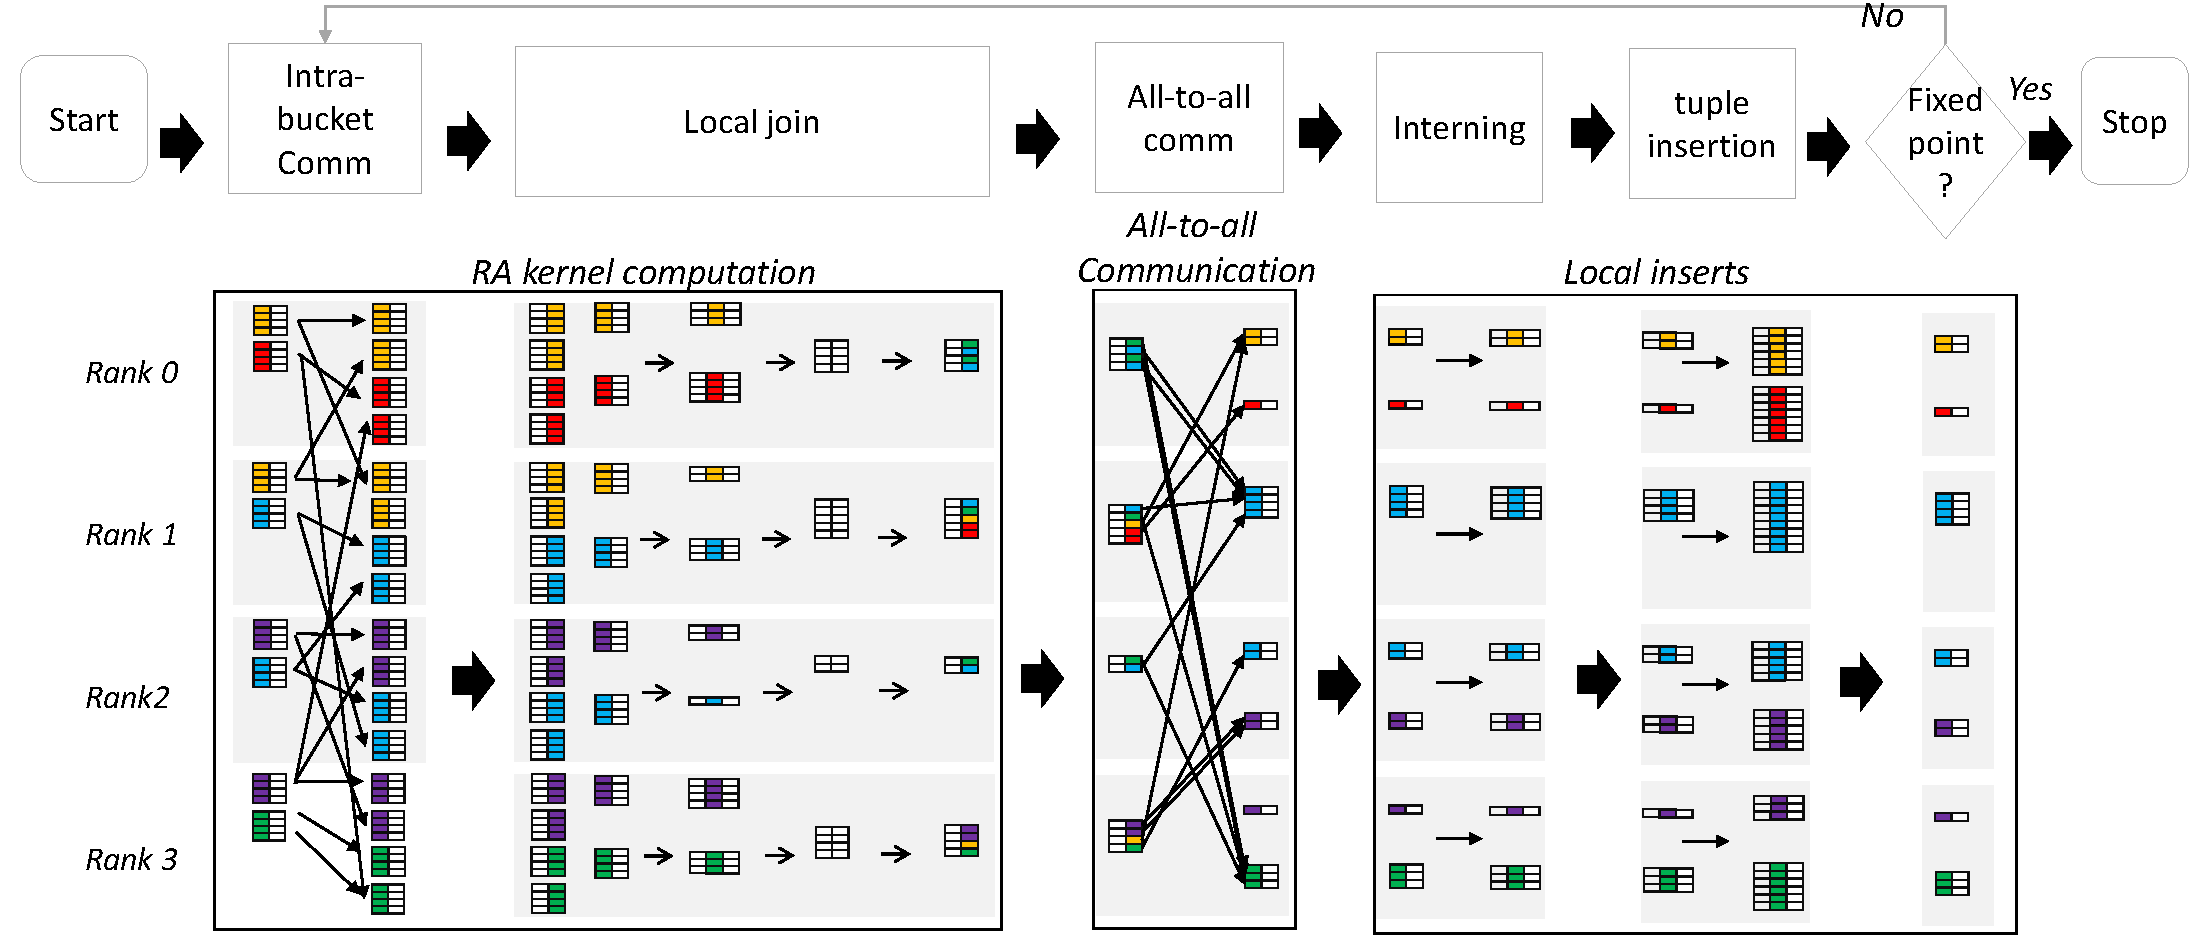
\includegraphics[width=0.99\textwidth]{fig/ra.pdf}
\caption{An illustration of the main phases of our parallel RA backend.}
\label{fig:sid}
\end{figure*}

\paragraph*{RA kernel computation}
The two-layered distributed approach, with local hash-based joins and hash-based distribution of relations, is a foundational method to distribute RA-kernel (primarily join) operations over many nodes in a networked cluster computer. This algorithm involves partitioning relations by their join-column values so that they can be efficiently distributed to participating processes~\cite{Valduriez:1988:PET:54616.54618}. The main insight behind this approach is that for each tuple in the outer relation, all relevant tuples in the inner relation must be hashed to the same MPI process or node, permitting joins to be performed locally on each process.

A major challenge with parallel workload partitioning is to ensure that every process gets to work on similar sized workloads that gives a load balanced system. A major challenge to enforce this load balance is to deal with inherently imbalanced data coming from key-skewed relations. To ensure uniform load across processes, we have built on previous approaches~\cite{kumar:hipc:2019, Kumar:2020} by developing strategies that mitigate load-imbalance in a dynamic manner. 
%First, we describe the architecture of our join (synthesized with projection and renaming for TC computation) in detail to ground this discussion. 
The approach~\cite{kumar:hipc:2019} uses a two-layered distributed hash-table to partition tuples over a fixed set of \emph{buckets}, and, within each bucket, to a dynamic set of \emph{subbuckets} which may vary across buckets. Each tuple is assigned to a bucket based on a hash of its key-column values, but within each bucket tuples are hashed on non-join-column values, assigning them to a local subbucket, then mapped to an MPI process. Within subbuckets, tuples are stored in B-trees, organized by key-column values. Our scheme permits buckets that have more tuples to be split across multiple processes, but requires some additional communication among subbuckets for any particular bucket. We have developed and evaluated a dynamic refinement strategy, to decide how many subbuckets to allocate per-bucket. To distribute subbuckets to managing processes, we use a round-robin mapping scheme which we found to be significantly more effective than hashing.

A join operation can only be performed for two \emph{co-located relations}: two relations each keyed on their respective join columns that share a bucket decomposition (but not necessarily a subbucket decomposition for each bucket). This ensures that the join operation may be performed separately on each bucket as all matching tuples will share a logical bucket; it does not, however, ensure that all two matching tuples will share the same subbucket as tuples are assigned to subbuckets (within a bucket) based on the values of non-join columns, separately for each relation.
The first step in a join operation is therefore an \emph{intra-bucket communication} (see Figure~\ref{fig:sid}) phase within each bucket so that every subbucket receives all tuples for the outer relation across all subbuckets (while the inner relation only needs tuples belonging to the local subbucket). Following this, a \emph{local join} operation (with any necessary projection and renaming) is performed in every subbucket.

\paragraph*{All-to-all communication}
To enable iterated parallel RA (in a fixed-point loop), processes must engage in a non-uniform all-to-all inter-process shuffle of generated tuples to their position in an output index.
This data exchange is performed to \emph{materialize} the output tuples generated from the local compute phase (where RA kernels are executed) to their appropriate processes (based on their bucket-subbucket assignment).
Materializing a tuple in an output relation (resulting from an RA operation) involves hashing on its join and non-join columns to find its bucket and sub-bucket (respectively), and then transmitting it to the process that maintains that bucket/sub-bucket.
As tuples generated from the local compute phase may each belong to an arbitrary bucket/sub-bucket in the output relation, an all-to-all communication phase is required to shuffle the output tuples to their managing processes.
Given variability in the number of tuples generated across processes, and in their destination processes (due to inherent imbalance), the communication phase in our framework is \emph{non-uniform} in nature.
The output tuples may each belong to an arbitrary bucket in the output relation, an MPI \emph{all-to-all} communication phase shuffles the output of all joins to their managing processes (preparing them for any subsequent iteration).

The overall scalability of the RA backend relies on the scalability of the all-to-all inter-process data exchange phase.
However, all-to-all is notoriously difficult to scale~\cite{4536141, scott1991efficient, thakur2005optimization}---largely because of the \emph{quadratic} nature of its workload. 
We address this scaling issue by adopting recent advancements~\cite{fan2022optimizing} that optimizes non-uniform all-to-all communication by extending the $\log$-time Bruck algorithm~\cite{bruck1997efficient, thakur2005optimization, traff2014implementing} for non-uniform all-to-all workloads. Traditional algorithms to implement non-uniform all-to-all communication takes linear iterations as every process must send and receive from every other process. Bruck algorithm however, sends more amount of data in logarithmic steps, and therefore significantly improves overall performance of all-to-all data exchange. Using the Bruck implementation of non-uniform all-to-all algorithm was instrumental in the overall scalibility of the backend.

\paragraph*{Local inserts}
After all-to-all data exchange, every process receives a new set of facts that must be materialized to be used as input in the subsequent iteration of the fixed-point loop. Local insert is a two-step process involving interning and inserting newly generated facts in the appropriate version of a relation (delta and total). Interning assigns a unique 64-bit key to every fact, and in order to scale this process, it must be is performed in an embarrassingly parallel manner without the need for any synchronization among processes. This is done by reserving the first 16 bits of the key for unique buckets ids, and the remaining 48-bits for facts. Since, a canonical-index (master index) bucket is never split across a process, reserving 16 bits for bucket ids ensures that globally unique intern keys can be created concurrently across processes. The fact-id component of the intern key is created by a bump pointer, which ensures that locally all facts receive a unique key. After interning, facts are added to their appropriate versions of the relations (delta or total), and a check is performed to see if a fixed-point has been reached. This check is performed by a global operation that checks the size of all relations across all processes, and if all sizes remains unchanged across two iterations, then this indicates that fixed-point has been attained and the program terminates, otherwise a new iteration is initiated.
